\section{Desarrollo Experimental 3}

Una forma habitual de expresar la potencia de salida de un amplificador es en dBm.  Lo
más sencillo para determinarla es emplear instrumentos con escalas en dB; por ejemplo,
un multímetro analógico como el siguiente:


\begin{figure}[H]
    \centering
    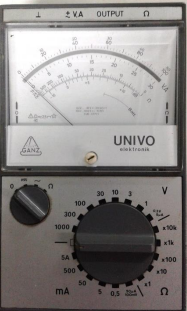
\includegraphics[width=0.25\textwidth]{images/voltimetroanalogico.png}
    \caption{multímetro analógico}
    \label{fig:conexiones}
\end{figure}

sin embargo hay que considerar que este instrumento de CA mide en dbu, por lo que es necesario convertir a dBm.
Para convertirlo hay que considerar que las mediciones estan calibradas para una impedancia de 600 ohms. Por lo que para convertir a dBm se debe usar la siguiente formula considerando la correcion correspondiente:
             

\begin{equation*}
    Correcion=10\log_{10}\left(\frac{600\Omega}{48\Omega}\right)=10,97dB
\end{equation*}

\begin{equation*}
    dBm=dbu+correcion
\end{equation*}

Por lo que procedemos a medir la potencia de salida del amplificador en dbu con el multímetro y luego convertimos a dBm usando la formula anterior.

\begin{figure}[H]
    \centering
    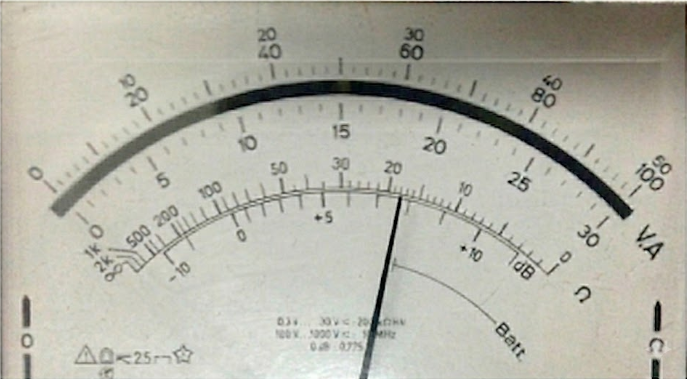
\includegraphics[width=0.50\textwidth]{images/voltimetroanalogicodbu.png}
    \caption{multímetro analógico dbu}
    \label{fig:conexiones}
\end{figure}
La medicion obtenida es de 7,7dbu , por lo que al convertir a dBm usando la formula anterior se obtiene:

\begin{equation*}
    dBm=dbu+correcion
\end{equation*}

\begin{equation*}
    dBm=7,7dbu+10,97dB=18,67dBm
\end{equation*}



Ahora para obetener la potencia de salida en watts se puede usar la siguiente formula:

\begin{equation*}
    dBm=10 \log_{10}\left(\frac{P}{1mW}\right)
\end{equation*}
 Que al despejar para P se obtiene:
\begin{equation*}
    Px=10^{\frac{dBm}{10}} \cdot 1mW
\end{equation*}

\begin{table}[H]
\centering
\resizebox{0.5\columnwidth}{!}{%
\begin{tabular}{|c|c|}
\hline
P (dBm) & Px (W) \\ \hline 
18,67dbm         & 73.72mW    \\  \hline  
\end{tabular}%
}
\end{table}


\section{Desarrollo Experimental 4}

Para medir la ganancia del amplificador, debe conectarse una carga equivalente a la que
se usará en condiciones normales de funcionamiento. En esta experiencia puede emplearse
el resistor $Rc1$, tal como quedó ajustado en la actividad anterior.

Si se comparan los valores de entrada y salida en dBu, la diferencia entre ambos corresponde
directamente a la ganancia de tensión del amplificador.

Si se desea obtener la ganancia de potencia, primero deben convertirse los dBu a dBm.
Para ello se necesitan los valores de $Rc1$ y $Re1$ medidos en los experimentos 1 y 2,
y luego aplicar la ecuación:

\begin{equation*}
    dBm=dbu+10\log_{10}\left(\frac{600\Omega}{Re1}\right)
\end{equation*}

Siguiendo el siguiente esquema de medicion obtenemos los distintos valores en dBu:

\begin{figure}[H]
    \centering
    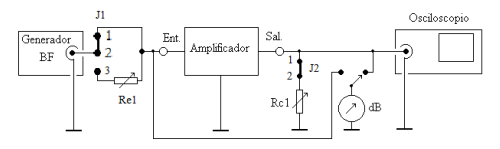
\includegraphics[width=0.50\textwidth]{images/ganancia.png}
    \caption{medicion de ganancia}
    \label{fig:conexiones}
\end{figure}

Logramos medir en la entrada 1,5dbu por lo que al convertir a dBm usando la formula anterior se obtiene:

\begin{equation*}
    dBm=dbu+10\log_{10}\left(\frac{600\Omega}{Re1}\right)
\end{equation*}

con una correccion de:

\begin{equation*}
    10\log_{10}\left(\frac{600\Omega}{48\Omega}\right)=10,97dB
\end{equation*}
\begin{equation*}
    dBm=1,5dbu+10,97dB=12,47dBm
\end{equation*}

\begin{table}[H]
\centering
\resizebox{0.75\columnwidth}{!}{%
\begin{tabular}{|c|c|c|}
\hline
F1   & (Salida) &   (Entrada)       \\ \hline 
1KHz & 7,7dbu   &                         1,5 dbu                         \\  \hline  
    & 18,67dbm  &                         12,47dbm           	            \\  \hline
\end{tabular}%
}
\end{table}


Ya teniendo el valor de entrada en dBm y el valor de salida que medimos anteriormente en dBu y posteriormente en dBm, se puede calcular la ganancia en dB usando la siguiente formula:

\begin{equation*}
    Ganancia=dBm_{salida}-dBm_{entrada}
\end{equation*}

\begin{equation*}
    Ganancia=18,67dBm-12,47dBm=6,2dB    
\end{equation*}

\begin{equation*}
    Ganancia=18,67dBu-12,47dBu=6,2dB    
\end{equation*}

Y tambien se puede calcular la ganancia en veces usando la siguiente formula:
\begin{equation*}
    Ganancia=\frac{V_{salida}}{V_{entrada}}
\end{equation*}

Para ello primero se deben convertir los valores de entrada y salida de dBu a voltaje usando la siguiente formula:

\begin{equation*}
    V=10^{\frac{dBu}{20}} \cdot 0,775V
\end{equation*}

Por lo que se obtiene:
\begin{equation*}
    V_{salida}=10^{\frac{7,7dbu}{20}} \cdot 0,775V=1,881V
\end{equation*}

\begin{equation*}
    V_{entrada}=10^{\frac{1,5dbu}{20}} \cdot 0,775V=0,921V
\end{equation*}

\begin{equation*}
    Ganancia_{veces} =\frac{V_{salida}}{V_{entrada}}=\frac{1,881V}{0,921V}=2,042
\end{equation*}


\begin{table}[H]
\centering
\resizebox{0.85\columnwidth}{!}{%
\begin{tabular}{|c|c|c|}
\hline
     & Ganancia (dB) & Ganancia (veces)   \\ \hline 
dBu     & 6.2           &    2.042          \\  \hline  
dBm     & 6.2           &          2.042      \\  \hline
\end{tabular}%
}

\end{table}

Ahora para sacar la incertidumbre en las mediciones en dbu se puede usar la siguiente formula:
\begin {equation*}
      \Delta dBu =\frac{8,68}{V_{medido}} \cdot \Delta V
\end{equation*}

\begin{equation*}
    \Delta V = \frac{Clase \cdot Rango}{100}=\frac{2,5\cdot 3V}{100}=0,075V
\end{equation*}
Para la salida se obtiene:
\begin{equation*}
    \Delta dBu =\frac{8,68}{V_{medido}} \cdot \Delta V= \frac{8,68}{1,881} \cdot 0,075V = 0,3462dB
\end{equation*}
Y para la entrada se obtiene:
\begin{equation*}
    \Delta dBu =\frac{8,68}{V_{medido}} \cdot \Delta V= \frac{8,68}{0,921} \cdot 0,075V = 0,706dB
\end{equation*}


\begin{table}[H]
\centering
\resizebox{0.85\columnwidth}{!}{%
\begin{tabular}{|c|c|}
\hline
           & Incertidumbre en dbu     \\ \hline 
Entrada    & $\pm$ 0.706                       \\ \hline  
Salida     & $\pm$ 0.3462                          \\ \hline
\end{tabular}%
}
\end{table}


